\chapter{Integration and Simulation}

\section{Introduction}
This chapter details the final stages of the project, focusing on how all previously designed systems were integrated, validated through digital simulation, and prepared for future development. It moves beyond theoretical design to practical implementation, demonstrating the seamless communication between the core components and presenting a comprehensive outlook on potential improvements.

\section{System Integration and Interfacing}
The success of the automated sorting cell relies on the synchronized operation of its hardware and software components. This section explains the critical communication links and data exchange mechanisms established between the PLC, the robotic arm, the HMI, and a Raspberry Pi acting as an additional control and data hub.

\subsection{The Communication Framework}
The primary communication protocol used for this project was \textbf{PROFINET}. As a robust and high-speed industrial Ethernet variant, PROFINET enabled real-time data exchange, ensuring that all components operated in perfect harmony. The network architecture, as shown in Figure \ref{fig:communication_diagram}, utilizes a router as a centralized point of communication that allows the Raspberry Pi, the PLC, the HMI, and the KUKA robot controller to interface seamlessly. This setup provides network flexibility and scalability for the cell's communication.

\begin{figure}[H]
    \centering
    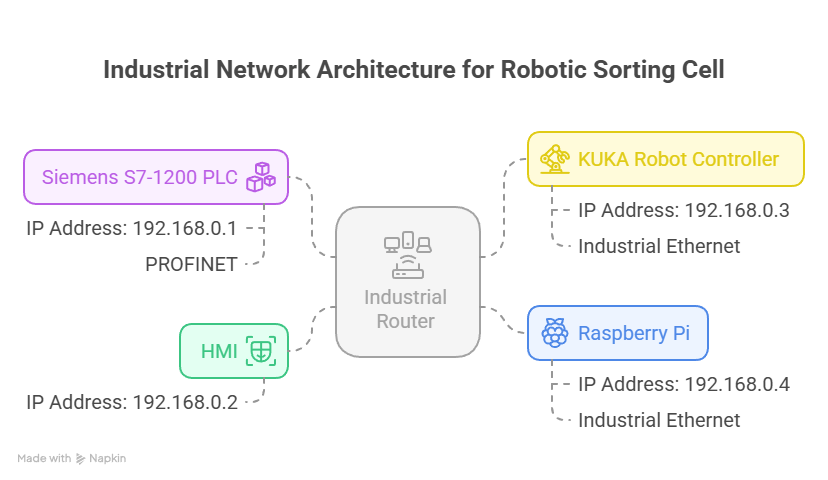
\includegraphics[width=0.8\textwidth]{Images/Chap4/communication_diagram.png}
    \caption{Communication diagram of the automated sorting cell.}
    \label{fig:communication_diagram}
\end{figure}

\subsection{Data Access via Python Scripting}
A crucial component of the system is the Raspberry Pi, which acts as a bridge between the vision system and the PLC. To facilitate this data exchange, a Python script was developed to communicate directly with the Siemens S7-1200 PLC. The script leverages a specialized library, such as \textbf{python-snap7}, an open-source Python wrapper for the Snap7 library, to establish a reliable TCP/IP connection to the PLC via the network router.

The script's primary function is to read from and write to the PLC’s dedicated \textbf{Data Blocks (DBs)}, which were pre-configured to store shared variables. Data is precisely addressed by its specific location within a DB, using the \textbf{DB number}, \textbf{byte offset}, and \textbf{bit offset}. This method is fundamental to the communication process, as it allows the script to directly manipulate variables in the PLC's memory.

For example, to read a variable, the Python script sends a command to the PLC specifying the DB number, the start byte, and the number of bytes to read. The PLC then sends the requested data back to the script. Conversely, to write a value, the script constructs a data packet containing the new value and the specific memory address, which the PLC then uses to update the corresponding variable.

This structured approach ensures that the Raspberry Pi can reliably provide the PLC with real-time data from the vision system, such as the CubeColor, thereby forming the core of the automated sorting logic. The ability to precisely read and write data at the byte level guarantees a robust and efficient communication link.

\begin{figure}[H]
    \centering
    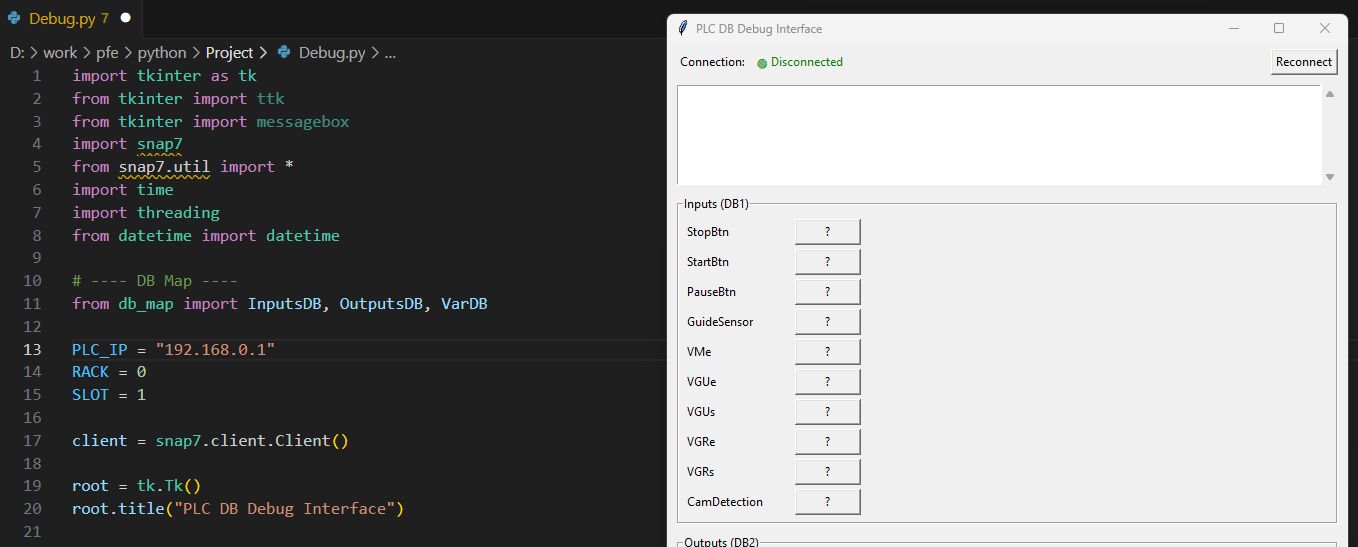
\includegraphics[width=1\textwidth]{Images/Chap4/python_interface.png}
    \caption{A Python-based interface for real-time PLC data access.}
    \label{fig:python_interface}
\end{figure}

\subsection{KUKA Robot Controller Interface}
The KUKA robotic arm's controller (KRC) is connected to the PLC via the PROFINET network and a central router. This network link allows the PLC to orchestrate the robot's movements by writing values to specific I/O addresses that are configured as shared data registers.

The robot's program is designed to continuously monitor these registers. For instance, the robot’s program looks for a change in the RobotPos variable. When the PLC writes a new value, the robot recognizes it as a command to move to a new position. After completing the move, the robot's program then writes a value to the RobotStatus register, informing the PLC that the task is complete and it is ready for the next command. This "read-then-write" mechanism is the foundation of the communication and coordination between the PLC and the robot.
\subsection{HMI Interface}
The HMI (Human-Machine Interface) is also connected to the router via PROFINET. It provides the operator with a graphical interface to interact with the system. The HMI's screens are linked to the PLC's variables, allowing it to:
\begin{itemize}
    \item \textbf{Display Real-Time Status:} Show the current state of the system, such as conveyor status, sensor feedback, and cube counts;
    \item \textbf{Receive Operator Commands:} Send commands to the PLC, such as START, STOP, or RESET, through on-screen buttons;
    \item \textbf{Monitor Alarms:} Display any system faults or warnings to the operator, enabling quick identification and resolution of issues.
\end{itemize}

\section{Digital Simulation and Verification}
Simulation was a cornerstone of this project, enabling comprehensive testing and validation of the entire system before physical implementation. This approach allowed for the early identification and resolution of potential issues, significantly reducing development time and minimizing risks. The simulation process was conducted across two distinct environments: the TIA Portal suite for automation logic and HMI, and a 3D modeling platform for physical and visual validation.

\subsection{TIA Portal Simulation}
The TIA Portal environment provides a powerful, integrated solution for simulating the entire control system before physical deployment. This process, often referred to as creating a \textbf{"digital twin" or "virtual commissioning"}, allows for a thorough, risk-free validation of the automation logic and network communication. The comprehensive simulation is carried out in a methodical, step-by-step manner.

First, the PLC's network settings are configured in the TIA Portal project. This includes assigning a specific IP address to the PROFINET interface of the virtual PLC. As shown in Figure \ref{fig:profinet_config}, the PLC is assigned the IP address \textbf{192.168.0.1}, which serves as its unique identifier on the network. This step is followed by compiling both the hardware configuration and the software to ensure there are no errors before the simulation begins.



The next critical step is to download the compiled program to the virtual PLC. The project is specifically downloaded to the \textbf{PLCSIM} instance, which acts as the simulated CPU. This ensures that the program is loaded into a virtual environment, allowing it to execute the control logic just as it would on a physical device. Once the download is complete, a connection is established between the TIA Portal engineering station and the virtual PLC, confirming that the simulation is online and ready for testing.
\begin{figure}[H]
    \centering
    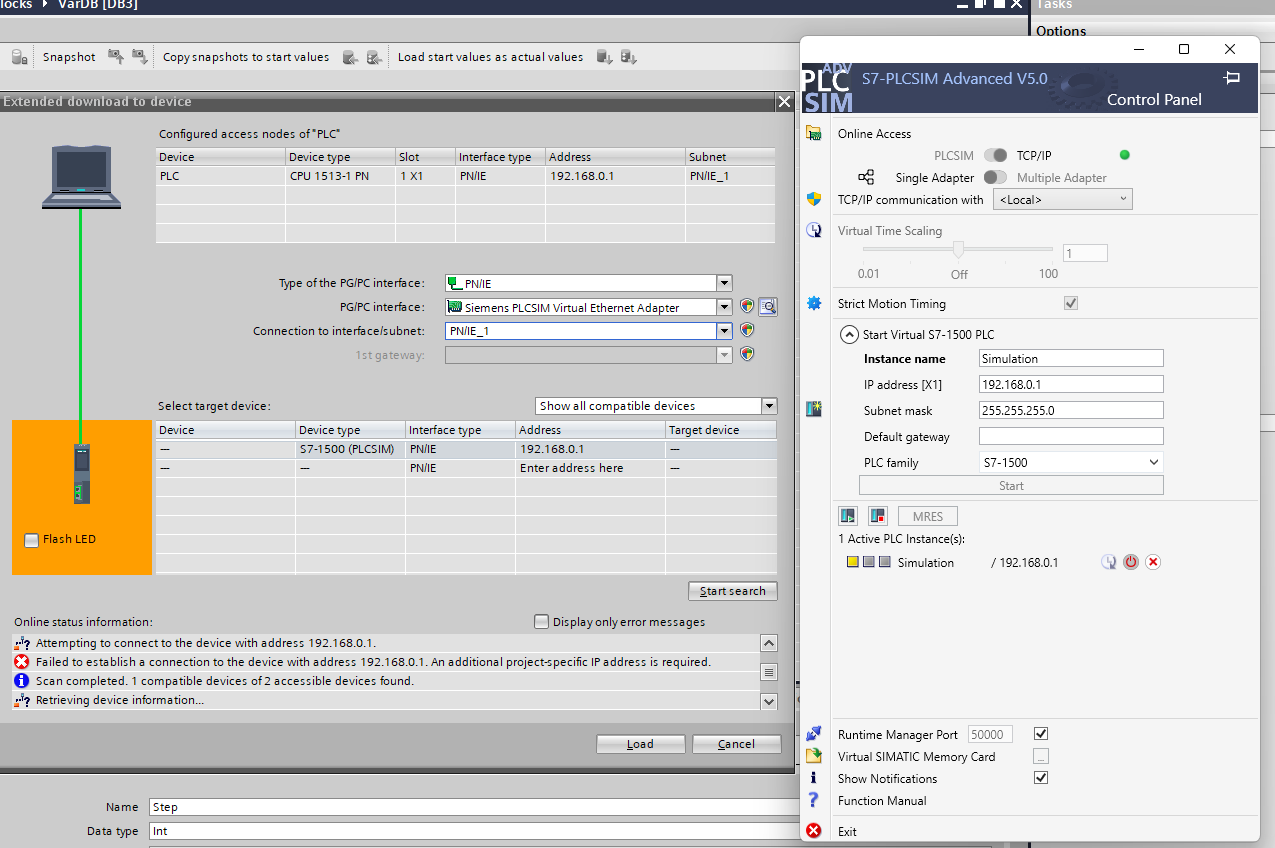
\includegraphics[width=0.9\textwidth]{Images/Chap4/PLC_PROFINET_Config.png}
    \caption{The PROFINET interface configuration to download the project in the simulated PLC.}
    \label{fig:profinet_config}
\end{figure}

With the PLC program running, the HMI can be simulated using \textbf{WinCC Unified}. TIA Portal automatically establishes a connection between the simulated HMI and the virtual PLC, allowing them to communicate in real time. This HMI can be accessed directly through a web browser, a key feature that allows for remote testing and validation of the user interface's operability. To access the interface, you first navigate to the specified IP address of the HMI in your browser, in this case, \textbf{192.168.0.2}. As the login page indicates, you must provide the correct user credentials to gain access to the control panel.

\begin{figure}[H]
    \centering
    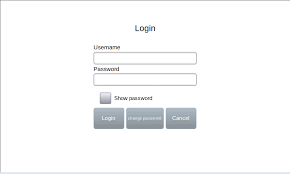
\includegraphics[width=0.6\textwidth]{Images/Chap4/HMI_Login_Page.png}
    \caption{The login page for the simulated HMI, accessible via a web browser.}
    \label{fig:hmi_login}
\end{figure}

Once logged in, the HMI provides a clear, visual interface with functional buttons and real-time data displays, enabling full interaction with the simulated system.

\begin{figure}[H]
    \centering
    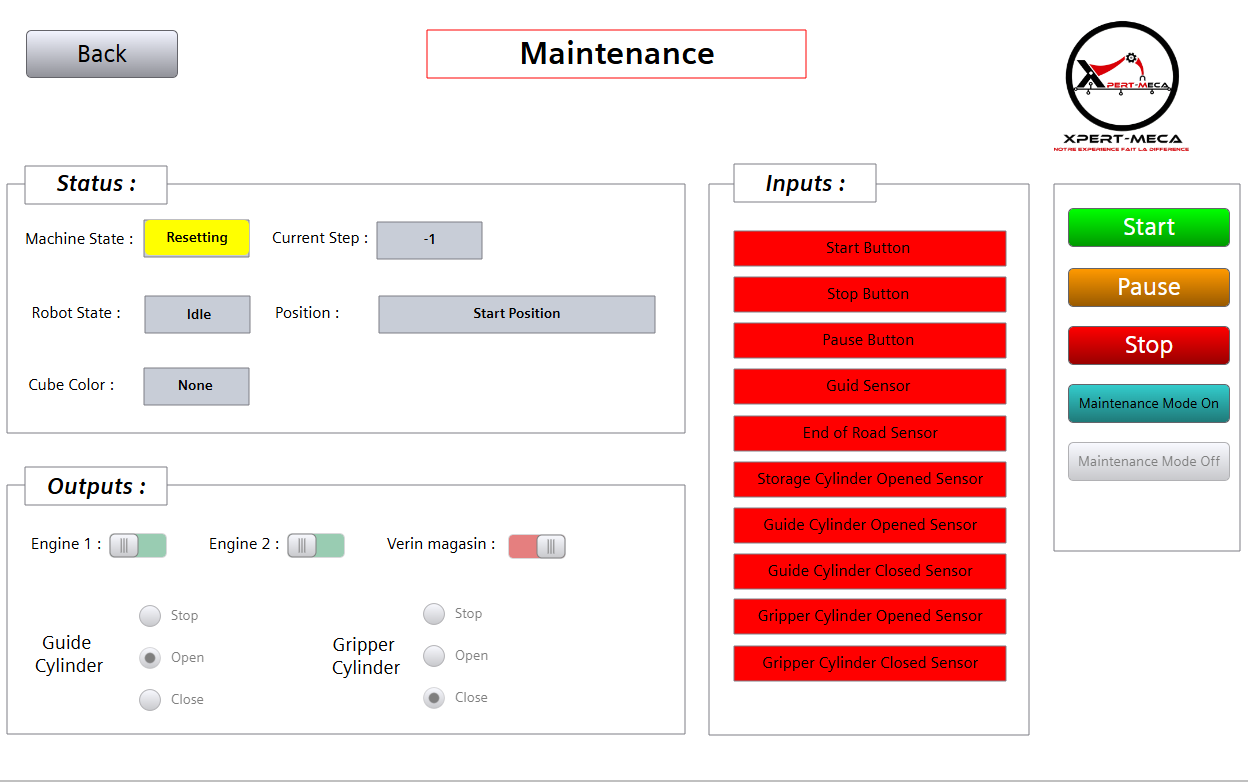
\includegraphics[width=0.8\textwidth]{Images/Chap4/HMI_Web_Simulation.png}
    \caption{The simulated HMI user interface with interactive elements.}
    \label{fig:hmi_web_simulation}
\end{figure}

To confirm the functionality of the system, all variables were monitored in real time. A crucial tool for this is the \textbf{Watch Table}, which provides a live view of the values of all internal tags and data blocks (DBs) on the virtual PLC. As seen in the watch table in Figure \ref{fig:watch_table}, variables like \textbf{`CubeColor`}, \textbf{`RobotPos`}, and \textbf{`RobotStatus` }update their values dynamically, proving that the control logic is executing correctly. This capability also allows for in-depth debugging by enabling a direct view into the logic, showing the status of each function block and its inputs and outputs, as demonstrated in Figure \ref{fig:online_diagnostics}.

\begin{figure}[H]
    \centering
    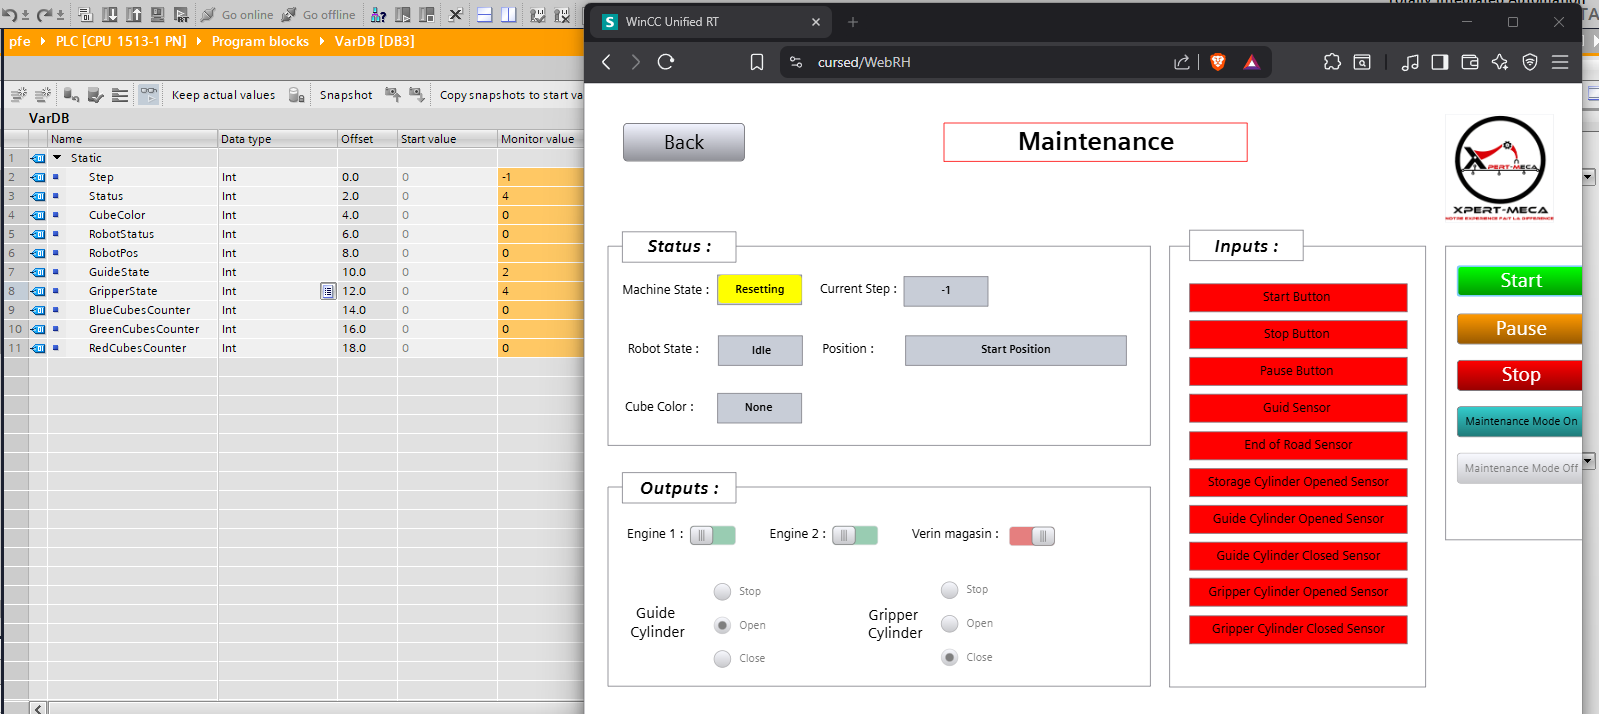
\includegraphics[width=1\textwidth]{Images/Chap4/Live_Watch_Table.png}
    \caption{The TIA Portal watch table, used to visualize and monitor real-time data from the PLC during simulation.}
    \label{fig:watch_table}
\end{figure}

\begin{figure}[H]
    \centering
    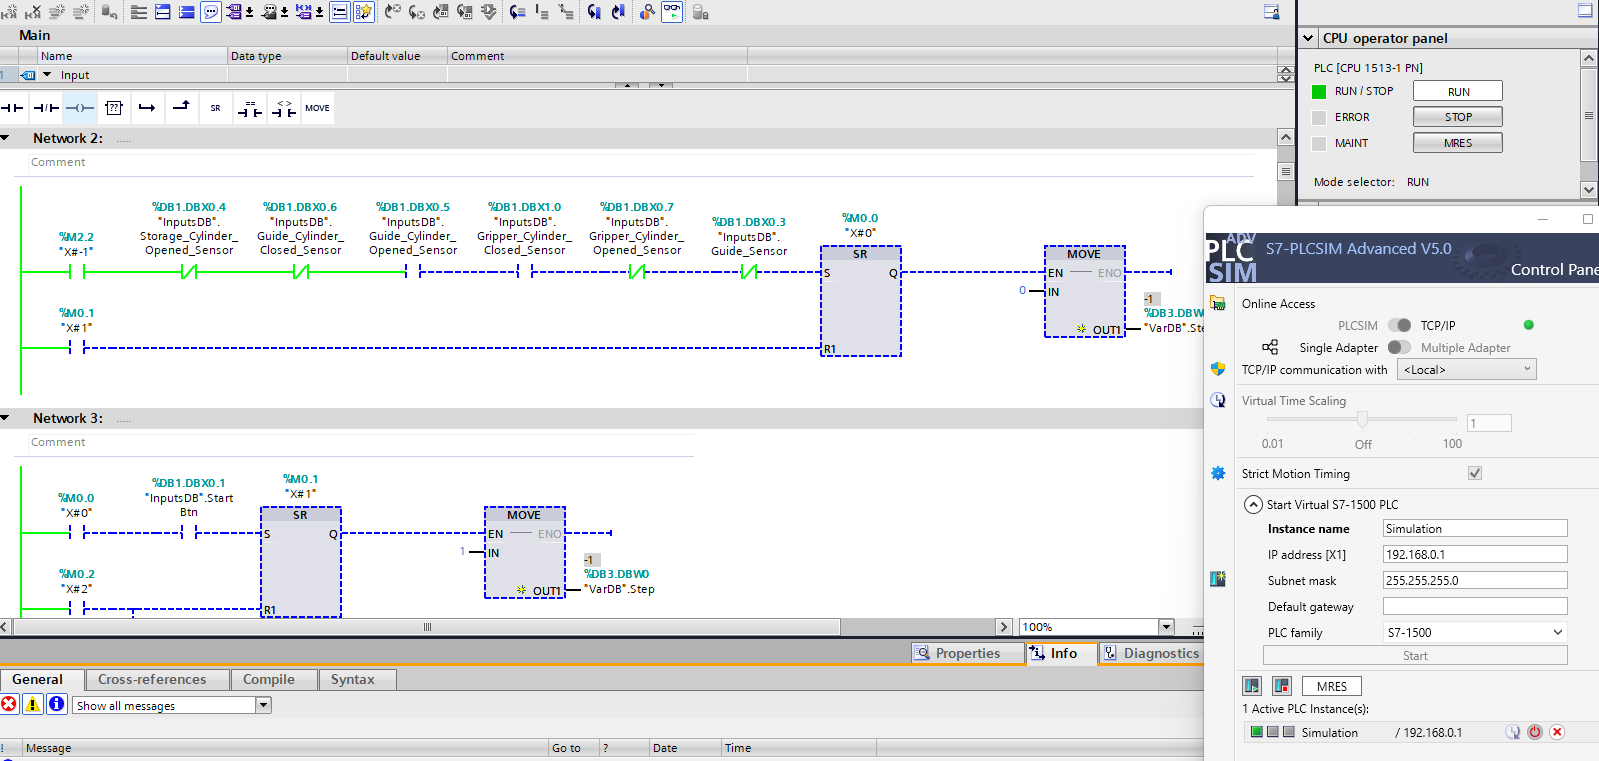
\includegraphics[width=1\textwidth]{Images/Chap4/Online_Diagnostics.png}
    \caption{Online diagnostics view of a function block, displaying the live values of its inputs and outputs.}
    \label{fig:online_diagnostics}
\end{figure}

\subsection{3D Simulation with Blender}
To create a realistic digital twin of the sorting cell, Blender was used to animate the system based on the control logic. The process involved several key steps:

\begin{itemize}
    \item \textbf{Model Optimization}: The original SolidWorks CAD models were imported into Blender. This process was critical, as the high-poly, detailed models were not suitable for a fluid animation workflow. To improve performance, the models were optimized by combining static parts (e.g., the frame and base) and reducing the overall number of components. This simplification made the project much more manageable and efficient for animation and rendering.
    
    \begin{figure}[H]
        \centering
        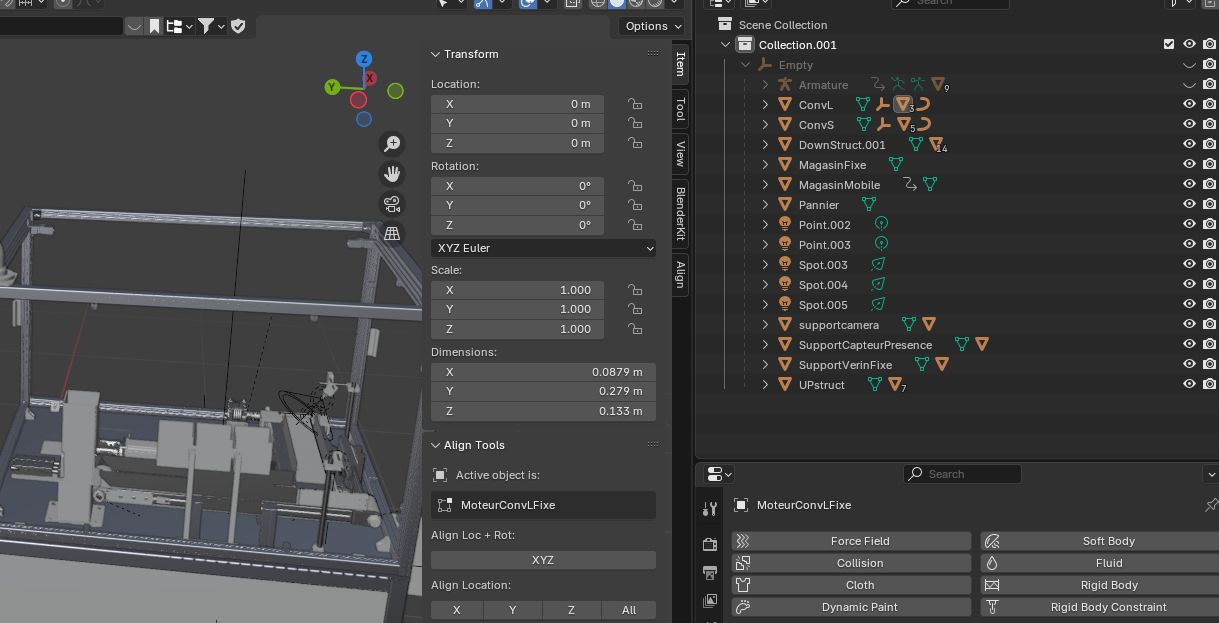
\includegraphics[width=0.9\textwidth]{Images/Chap4/Blender_Optimization.png}
        \caption{Blender collection parts}
        \label{fig:blender_optimization}
    \end{figure}
    
    \item \textbf{Texturing}: After optimization, realistic materials and textures were added to the models to visually represent the final appearance of the cell. As shown in Figure \ref{fig:blender_texturing}, this included applying appropriate colors and finishes to mimic painted metal, rubber, and other materials. This step was crucial for enhancing the visual fidelity of the simulation and creating a convincing representation of the physical cell.

    \begin{figure}[H]
        \centering
        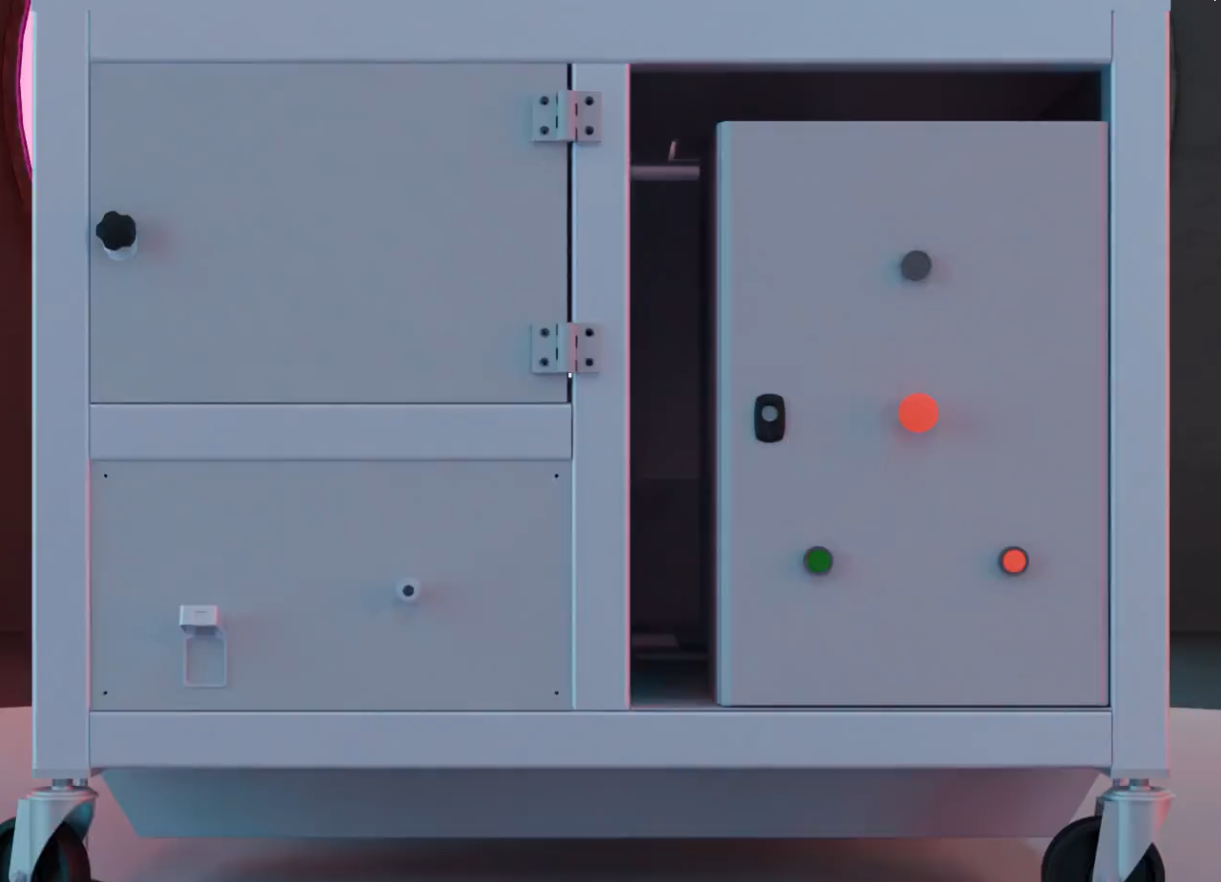
\includegraphics[width=0.6\textwidth]{Images/Chap4/Blender_Texturing.png}
        \caption{The 3D model in Blender with realistic materials and textures.}
        \label{fig:blender_texturing}
    \end{figure}

    \item \textbf{Physics and Rigging}: Physics simulations were applied to components that interact with the cubes, such as the conveyor belt and sorting mechanism, ensuring realistic behavior. This simulation was crucial for accurately depicting how the cubes would behave as they moved through the cell. Additionally, the robotic arm was \textbf{"rigged"} with a bone structure. This process of creating a digital skeleton allowed for the precise animation of the arm's joints and end-effector, ensuring that its movements accurately mimicked those controlled by the PLC. As seen in Figure \ref{fig:blender_rigging}, the rig provides a framework for animating the arm's complex movements.

    \begin{figure}[H]
        \centering
        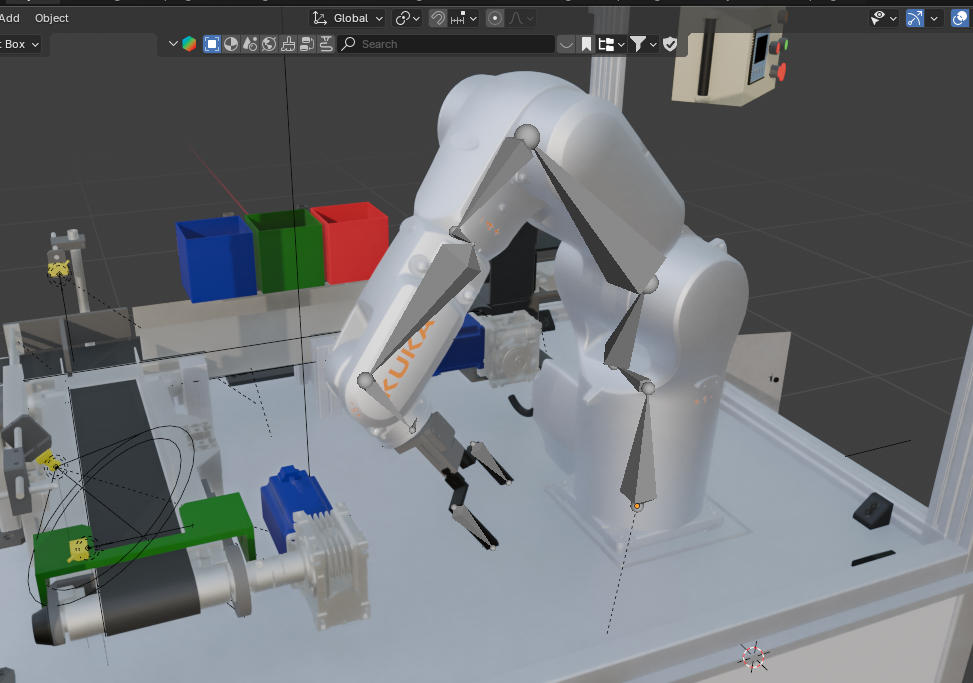
\includegraphics[width=0.6\textwidth]{Images/Chap4/Blender_Rigging.png}
        \caption{Robotic arm's bone structure.}
        \label{fig:blender_rigging}
    \end{figure}

    \item \textbf{Animation and Presentation}: The final step was to animate the complete sorting cycle from start to finish. This process involved synchronizing the rigged robotic arm and the physics-simulated cubes with the logical sequence defined in the PLC program. As demonstrated in Figure \ref{fig:blender_animation}, this detailed visual representation of the entire process served as a powerful tool for showcasing the project's functionality and for identifying any motion-related design flaws. The final rendered animation was used for both project verification and presentation purposes.

    \begin{figure}[H]
        \centering
        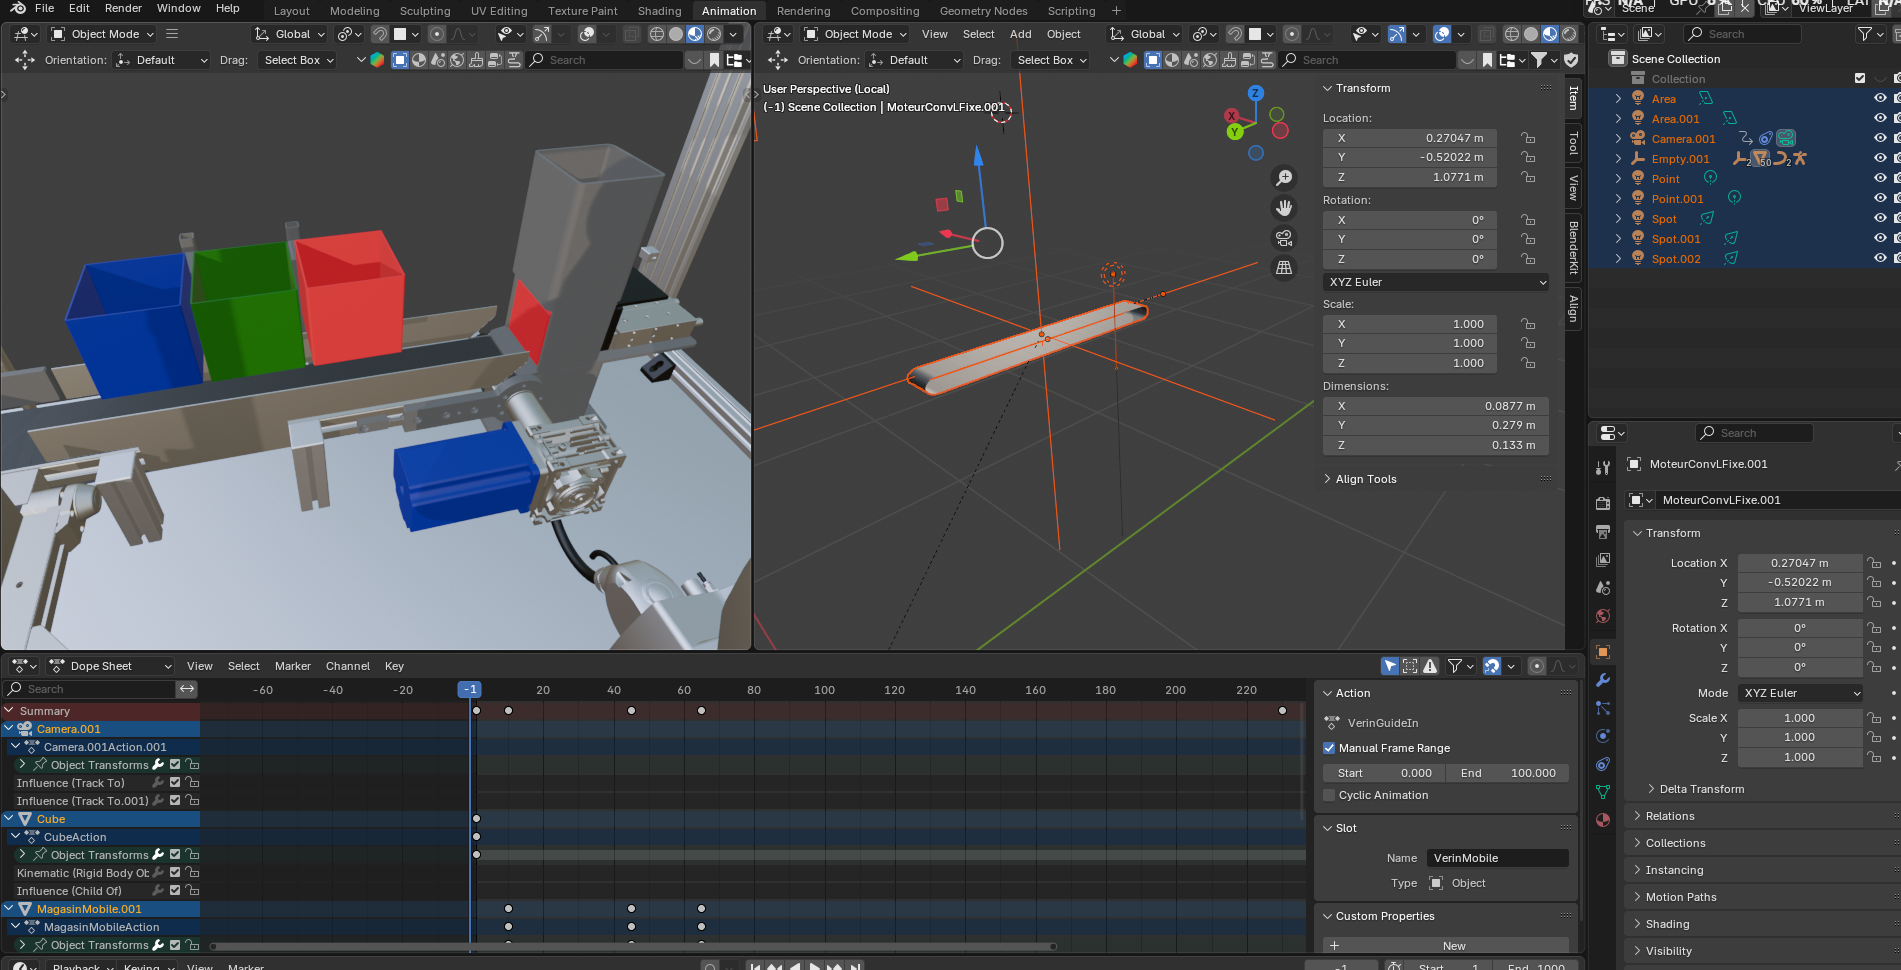
\includegraphics[width=1\textwidth]{Images/Chap4/Blender_Animation.png}
        \caption{Blender animation window and timeline}
        \label{fig:blender_animation}
    \end{figure}
\end{itemize}


\section{Conclusion}
This chapter successfully demonstrated the transition from theoretical design to a functional and verifiable system through advanced simulation. By meticulously detailing the PROFINET communication network, we established a clear link between the PLC, Raspberry Pi, and KUKA robot, highlighting the central role of a network router in orchestrating seamless data exchange. We then delved into the crucial process of virtual commissioning, showcasing how TIA Portal and Blender were used to create a comprehensive digital twin. This approach allowed for the rigorous testing of both the control logic and HMI functionality, as well as the accurate visualization of the cell's physical movements. The structured methodology presented here—from network configuration to real-time variable monitoring—is fundamental to the development of a predictable, efficient, and safe robotic sorting solution.